\documentclass[a4paper, 12pt]{article}

\usepackage{hyperref}
\usepackage{fullpage}
\usepackage[top=0.5in, bottom=1.5in, left=0.5in, right=0.5in, footskip=4em]{geometry}
\usepackage{amsmath}
\usepackage{fancyhdr}
\usepackage[usenames,dvipsnames]{xcolor}
\usepackage{pgfornament}

\usepackage[shortlabels]{enumitem}
\usepackage{xspace}
\usepackage{lastpage}
\usepackage{multicol}
\usepackage{blindtext}
\usepackage{titling}
\usepackage{standalone}
\usepackage{amsfonts}
\usepackage[framemethod=TikZ]{mdframed}
\usetikzlibrary{calc}
\usepackage{lineno}
\usepackage{amsthm}
\usepackage{amssymb}
\usepackage{mathtools}
\usepackage{datetime}
\usepackage[most]{tcolorbox}
\usepackage{cancel}
\usetikzlibrary{tikzmark}
\usepackage{pgfplots}
\linenumbers


%BEGIN_FOLD Commands
\newcommand{\half}{\frac{1}{2}}
\newcommand{\epv}[1]{\ensuremath{\left< #1 \right>}\xspace}
\newcommand{\variance}{\ensuremath{\text{Var}}}
\newcommand{\eout}{\ensuremath{E_\text{out}}\xspace}
\newcommand{\ein}{\ensuremath{E_\text{in}}\xspace}
\newcommand{\cx}{\ensuremath{\mathcal{X}}\xspace}
\newcommand{\cz}{\ensuremath{\mathcal{Z}}\xspace}
\newcommand{\real}{\mathbb{R}}
\DeclareSymbolFont{extraup}{U}{zavm}{m}{n}
\DeclareMathSymbol{\varheart}{\mathalpha}{extraup}{86}
\DeclareMathSymbol{\vardiamond}{\mathalpha}{extraup}{87}
\renewcommand{\heartsuit}{\textcolor{red}{\varheart}}
\renewcommand{\diamondsuit}{\textcolor{red}{\vardiamond}}
\newcommand{\definition}{\vspace{1em}\noindent\textbf{Def:} }
\newcommand{\theorem}{\vspace{1em}\noindent\textbf{Theorem:} }
\newcommand{\example}{\vspace{1em}\noindent\textbf{Example:} }
\newcommand{\predicate}{\vspace{0.25em}\noindent\textbf{Inductive Predicate:} }
\newcommand{\inductivestep}{\vspace{0.25em}\noindent\textbf{Inductive Step:} }
\renewcommand{\proof}{\vspace{0.5em}\noindent\textbf{Proof:} }
\newcommand{\lemma}{\vspace{1em}\noindent\textbf{Lemma:} }
\newcommand{\hint}{\textbf{Hint:} }
\newcommand{\basecase}{\vspace{0.25em}\noindent\textbf{Base Case:} }
\newcommand{\inductivehypothesis}{\vspace{0.25em}\noindent\textbf{Inductive Hypothesis:} }
\newcommand{\collorary}{\vspace{1em}\noindent\textbf{Collorary:} }
\newcommand{\qedd}{\qed\newline}
\newcommand{\kwd}[1]{\textcolor{blue}{\textbf{\underline{#1}}}}
\newcommand\ColorBox[2][]{%
	\stepcounter{mybox}%
	\node[draw=red!70!black,fill=red!20,align=left,#1] (box\themybox) {#2};
}
\newcommand{\expl}[2]{%
	\underset{\substack{\uparrow\\\mathrlap{\text{\hspace{-1em}#2}}}}{#1}}
\newcommand{\uexpl}[2]{%
	\overset{\substack{\mathrlap{\text{\hspace{-1em}#2}}\\\downarrow}}{#1}}
\newcommand{\st}{\text{ such that }}
\newcommand{\R}{\textcolor{red}{R}}
\newcommand{\sumn}{\sum^n_{i=0}}
\newcommand{\sumxn}{\sum^n_{x=0}}
%\newcommand{\qed}{\ensuremath{\blacksquare}}
%END_FOLD
\newcommand{\sidenote}[1]{\textcolor{gray}{#1}}

%BEGIN_FOLD miscellaneious default
\makeatletter
% Make a copy of macros responsible for entering display math mode
\let\start@align@nopar\start@align
\let\start@gather@nopar\start@gather
\let\start@multline@nopar\start@multline
% Add the "empty line" command to the macros
\long\def\start@align{\par\start@align@nopar}
\long\def\start@gather{\par\start@gather@nopar}
\long\def\start@multline{\par\start@multline@nopar}
\makeatother
\setlength{\columnsep}{1cm}
%opening
\setlength{\abovedisplayskip}{-\baselineskip}%
\setlength{\abovedisplayshortskip}{\abovedisplayskip}%

\pagestyle{fancy}
\renewcommand{\headrulewidth}{0pt}
\lfoot{\small{\course}: Week \weekno}
\rfoot{\small{\thetitle}}
\rhead{}
\cfoot{\pgfornament[height=1em, ydelta=-0.4em]{17} \thepage of \pageref{LastPage}  \pgfornament[height=1em, ydelta=-0.4em]{18}}

\DeclareMathOperator{\sign}{sign}
\newcommand{\vect}[1]{\ensuremath{\mathbf{#1}}\xspace}

\tikzstyle{every picture}+=[remember picture]
\newcommand{\bwgrid}[1]{
	\def \aaa #1
	
	\foreach \y in {0,1,2} {
		\foreach \x in {0,1,2} {
			\pgfmathsetmacro{\clr}{\aaa[\x][\y]}
			%\message{aaa \clr}
			\definecolor{MyColor}{rgb}{\clr,\clr,\clr}
			\path[fill=MyColor] (\x,\y) rectangle ++(1,1); 
		}
	}
	\draw[step=1cm,very thin] (0,0) grid (3,3);	
}

\setenumerate{label=\alph*.)}
\definecolor{db}{RGB}{100,65,23}

%END_FOLD

\newcommand{\course}{Discrete Math}
\title{Sum and Asymptotics}
\newcommand{\weekno}{4}

\begin{document}
\begin{center}
	\textcolor{orange}{\textsc{\course}}\\
	\huge\textbf{\textsc{\thetitle}}\\
	\small\textcolor{gray}{Last updated:\, \today \, \currenttime}\\
	\pgfornament[width=0.7\textwidth, color=white!30!black]{88}
\end{center}

\begin{multicols}{2}
\section*{Time Value of Money}
Suppose I offer you two choices.
\begin{enumerate}
	\item 1 Million Baht now.
	\item 1,100,000 Baht 10 years from now.
\end{enumerate}
Which one is a better choice?

An important factor in deciding between the two is the interest rate($r$). What we need to compare is if we get 1 Million Baht now and put it safe in the bank how much is would it be in the next 10 years.

After 1 year, your 1 Million Baht will become
\[
	1,000,000 \xrightarrow{\text{1 year}}	(1+r)\times 1,000,000
\]

Then, 1 year later(on your 2nd year).
\[
	(1+r)1,000,000 \xrightarrow{\text{1 more year}}	(1+r)^2\times 1,000,000
\]

This means after 10 years your 1,000,000 Baht will become
\[
1,000,000 \xrightarrow{\text{10 years}}	(1+r)^{10}\times 1,000,000
\]

The current interest rate is at 2\%. This means $r = 0.02$. So after 10 years the value of 1,000,000 Baht is
\[
1,000,000 \times (1.02)^{10} = 1,218,994
\]

So, we can conclude that the 1,000,000 is a better deal because the value of both deals 10 years from now of the first deal is better than the second one.

In the previous analysis, we compared the future value of the money together. We can look at this from another angle by comparing the \kwd{present value}(PV) of the deal instead.

The present value of the first deal is easy. The present value of 1,000,000 Baht now is, by definition, 1,000,000.

For the second deal, we need to find how much 1,100,000 Baht next 10 year worth now. What we need to find is how much money do we need today to put in the bank so that we will get 1,100,000 Baht in the next 10 year.
\[
	PV_{1.1M, 10year} \times (1+r)^{10} = 1,100,000
\]

So, the present value of 1.1M Baht 10 year from now is
\[
	PV_{1.1M, 10year} = \frac{1,100,000}{(1+r)^{10}} = 902,383
\]

Or, in general,
\[
	PV_{m, t} = \frac{m}{(1+r)^t}.
\]

So, the first deal is much better.

\section*{Monthly Interest Rate}

Before we go to the next topic let us think about how to calculate monthly interest rate. We can just equate the money after 1 yearly interest rate and the money after 12 monthly interest payment.
\[
	M_0 (1+r_y) = M_0(1+r_m)^{12}
\]

Thus,
\[
	r_m = (1+r_y)^{\frac{1}{12}}-1
\]

For example, at the current 0.02 interest rate. The monthly interest rate is 0.00165.

\section*{Geometric Sum}

Let us consider a bit more complicated deal. Supposed you are buying a car of 1,000,000 Baht and the dealer give you two choices
\begin{enumerate}
	\item Pay cash now and you will get 40,000 Baht discount.
	\item Or you can pay 20,000 per month for 50 months.
\end{enumerate}
Which deal should you take given that you have enough cash now?

The real question we need to decide is whether the present value of paying 20k for 50 months is. The present value of this deal is just the sum of the present value of each payment.

Let us label each payment from 0 to 49 where 0th payment indicate the payment now at month 0 and the nth payment is the payment n-month in the future.

The present value of the nth payment is given by
\[
	\frac{20,000}{(1+r_m)^{n}}.
\]

So, the sum of the total payment is given by
\[
	\frac{20,000}{(1+r_m)^{0}} + \frac{20,000}{(1+r_m)^{1}} + \frac{20,000}{(1+r_m)^{2}} \ldots + \frac{20,000}{(1+r_m)^{49}}
\]

Factoring out the 20,000
\begin{align*}
	20,000\left(\frac{1}{(1+r_m)^{0}} +\ldots+ \frac{1}{(1+r_m)^{49}} \right)
\end{align*}

So we will need to evalute the sum that looks like
\[
S = 1 + x + x^2 + x^3 + \ldots x^{49} = \sum_{i=0}^{i=49} x^i
\]

The sum above is called geometric sum. The $\sum$ symbol reads sigma is the notation for the sum. This is one of the few sums that has a closed form formula. Finding the closed form formula is quite simple using the method of purtabation.
\begin{align*}
	S &= 1 + x + x^2 + \ldots + x^m
\end{align*}
multiplying by $x$ on both sides
\begin{align*}
	Sx &= x + x^2 + x^3 + \ldots + x^m + x^{m+1}\\
	Sx &= S-1 + x^{m+1}
\end{align*}
Grouping $S$
\begin{align*}
	S(x-1) &= x^{m+1} - 1\\
	S &= \frac{x^{m+1} - 1}{x-1}\\
\end{align*}
Which means
\begin{equation}
1 + x + x^2 + \ldots + x^m = \frac{x^{m+1} - 1}{x-1}
\label{eq:geosum}
\end{equation}

In our case,
\[
	x = \frac{1}{1+r_m} = 0.99835
\]
Thus,
\[
\frac{1}{(1+r_m)^{0}} +\ldots+ \frac{1}{(1+r_m)^{49}} = 48.311
\]

So, the present value of the 50 payment is 960,621. But, the present value of the cash payment is only 960,000. So, paying cash now is a slightly better deal.

So, by the time you get your own car, show me that you learn something from this course and do the calculation first.

\section*{Infinite Geometric Sum}

We can consider Equation \ref{eq:geosum} in the case where we sum it up to infinity. If $|x|<1$, then the sum becomes
\[
	\sum_{i=1}^{\infty}x^i = \frac{1}{1-x}
\]

\section*{Saving Money}
Suppose after you graduate you save 10K a month and put it in the bank. How much do you have after 5 years? This is left for the reader as an exercise. All you need to do is to write out what happen to the 10k you put in at i-th month at the end of 5 years.

\end{multicols}
\section*{Variation on Geometric sum}

Consider
\[
	\sum^{n}_{i=1} ix^i = 1x + 2x^2 + 3x^3 + \ldots
\]

You can actually find this sum quite easily by just differentating both side of Equation \ref{eq:geosum} with respect to $x$ and manipulating the expression a little bit. Specifically,
\begin{align*}
1 + x^2 + x^3 + \ldots + x^m &= \frac{x^{m+1}-1}{x-1}\\
\frac{d}{dx} \left( 1 + x + x^2 + x^3 + \ldots + x^m \right) &= \frac{d}{dx} \left(\frac{x^{m+1}-1}{x-1}\right)\\
0 + 1+ 2x + 3x^2 + \ldots + mx^{m-1} &= \frac{(x-1)(m+1)x^m +x^{m+1}-1 }{(x-1)^2}\\
0 + 1 + 2x + 3x^2 + \ldots + mx^{m-1} &= x^m \left(\frac{m+1}{x-1}\right)  -\frac{x^{m+1}-1}{(x-1)^2}\\
0 + x + 2x^2 + 3x^3 + \ldots + m x^m & = x^{m+1} \left(\frac{m+1}{x-1}\right)  -x\frac{x^{m+1}-1}{(x-1)^2}
\end{align*}

If you ever need something like
\[
	\sum^{n}_{i=1} i^2x^i = 1x + 2^2x^2 + 3^2x^3 + \ldots
\]
All we need to do is just keep differentiating it. 
\begin{multicols}{2}
\section*{Sum Properties}
Here are some obvious property of sum. All of them are obvious if you just write it out.

First, let us consider multiplying a constant to a sum
\[
    \sum_{i=0}^n 5 i  = 5\times 1 + 5\times 2 + 5\times 3 + 5\times 4 + \ldots
\]
We can see that if we write it out we can just factor out the 5 from each term. We can then conclude that we can just pull the constant out from the sum.
\[
    \sum_{i=0}^n c f(i) = c \times  \sum_{i=0}^n f(i)
\]

Let us consider another situation where we add the terms in the sum:
\begin{align*}
    \sumn \left(i^2 + i\right) &= 1^2 + 1 + 2^2 + 2 + 3^2 + 3 + \ldots\\
    &= 1^2 + 2^2 + 3^2 + \ldots + 1 + 2 + 3 + \ldots\\
    &= \sumn i^2 + \sumn i
\end{align*}
So, we can also distribute the sum inside the expression.
\[
    \sumn f(i) + g(i) = \sumn f(i) + \sumn g(i)
\]

One thing that students get wrong a lot eventhough it looks trivial is the sum of constants:
\[
	\sum_{i=1}^n 3 = \underbrace{3 + 3 + 3 + \ldots + 3}_{\text{There are $n$ of these}} = 3n.
\]
So, the answer is $3n$ not 3.

However, it is quite easy to see that the sum doesn't expand for the product.
\[
    \sumn f(i)g(i) \ne \left(\sumn f(i)\right) \times \left(\sumn g(i)\right)
\]
The counter example for this is left for the reader as an exercise.

\section*{Integral Bound}
The geometric sum we consider above is one of a very few sum that has a closed form. The sum, in general, has no closed form formula. For example, let us consider
\[
    \sum_{x=1}^{9} \frac{1}{\sqrt{x}} = \frac{1}{\sqrt{1}} + \frac{1}{\sqrt{2}} + \frac{1}{\sqrt{3}}+ \ldots+ \frac{1}{\sqrt{9}} 
\]

This sum has no close form but first let us consider what exactly does the sum represent. We can draw number of bars of width 1 and each with height equal to $\frac{1}{\sqrt{x}}$ where $x$ is the right side $x$ position. This is shown with blue bars below.

\pgfplotsset{compat=1.8}
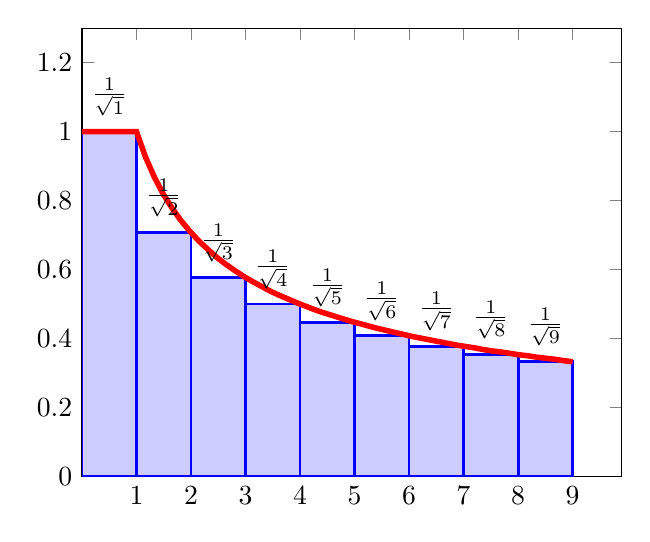
\begin{tikzpicture}
\begin{axis}[xmin=0, ymin=0, ymax=1.3, xtick={1,2,3,4,5,6,7,8,9}]
\addplot[blue, line width=1, ybar, bar width = 1, bar shift=-0.5, fill = blue!20!white, ] plot coordinates
	{(1, 1.000)
	(2, 0.707)
	(3, 0.577)
	(4, 0.500)
	(5, 0.447)
	(6, 0.408)
	(7, 0.378)
	(8, 0.354)
	(9, 0.333)};

\addplot[red, line width=2] plot coordinates
{
(0, 1)
(1.000, 1.000)
(1.163, 0.927)
(1.327, 0.868)
(1.490, 0.819)
(1.653, 0.778)
(1.816, 0.742)
(1.980, 0.711)
(2.143, 0.683)
(2.306, 0.659)
(2.469, 0.636)
(2.633, 0.616)
(2.796, 0.598)
(2.959, 0.581)
(3.122, 0.566)
(3.286, 0.552)
(3.449, 0.538)
(3.612, 0.526)
(3.776, 0.515)
(3.939, 0.504)
(4.102, 0.494)
(4.265, 0.484)
(4.429, 0.475)
(4.592, 0.467)
(4.755, 0.459)
(4.918, 0.451)
(5.082, 0.444)
(5.245, 0.437)
(5.408, 0.430)
(5.571, 0.424)
(5.735, 0.418)
(5.898, 0.412)
(6.061, 0.406)
(6.224, 0.401)
(6.388, 0.396)
(6.551, 0.391)
(6.714, 0.386)
(6.878, 0.381)
(7.041, 0.377)
(7.204, 0.373)
(7.367, 0.368)
(7.531, 0.364)
(7.694, 0.361)
(7.857, 0.357)
(8.020, 0.353)
(8.184, 0.350)
(8.347, 0.346)
(8.510, 0.343)
(8.673, 0.340)
(8.837, 0.336)
(9.000, 0.333)
};

\node() at (axis cs: 0.5000,1.1000){$\frac{1}{\sqrt{1}}$};
\node() at (axis cs: 1.5000,0.8071){$\frac{1}{\sqrt{2}}$};
\node() at (axis cs: 2.5000,0.6774){$\frac{1}{\sqrt{3}}$};
\node() at (axis cs: 3.5000,0.6000){$\frac{1}{\sqrt{4}}$};
\node() at (axis cs: 4.5000,0.5472){$\frac{1}{\sqrt{5}}$};
\node() at (axis cs: 5.5000,0.5082){$\frac{1}{\sqrt{6}}$};
\node() at (axis cs: 6.5000,0.4780){$\frac{1}{\sqrt{7}}$};
\node() at (axis cs: 7.5000,0.4536){$\frac{1}{\sqrt{8}}$};
\node() at (axis cs: 8.5000,0.4333){$\frac{1}{\sqrt{9}}$};
\end{axis}
\end{tikzpicture}

From the figure, we can see that the sum we want to calculate is just the area of the blue bars. This is be cause the the area of i-th bar is exactly $1\times \frac{1}{\sqrt{x}}$.

Even though there is no closed form formula for this sum we can see from the figure that the area of the blue bars is \emph{less than} the area under the red line. The red line(ignoring the first parts) is given simply by
\[
	\textcolor{red}{f(x)} = \frac{1}{\sqrt{x}}
\]
You can try a few points to see that this is indeed correct.

So we know that
\begin{align*}
	\sum_{x=1}^{9} \frac{1}{\sqrt{x}} &\le \int\limits_{x=1}^{x=9} \frac{1}{\sqrt{x}} dx + 1\times \frac{1}{\sqrt{1}}\\
	&\le \left. 2 x^\half\right \vert_{x=1}^{x=9} + 1\\
	&\le 2\left(3-1 \right) + 1\\
	&\le 5
\end{align*}
where the last term comes from the area under the first flat red region.

We can do a similar trick for lower bound of the sum by considering a similar line just right below the blue bars.
\pgfplotsset{compat=1.8}
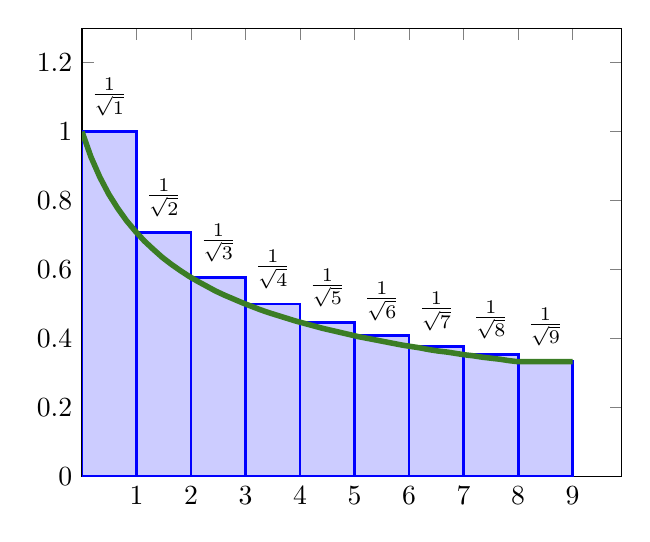
\begin{tikzpicture}
\begin{axis}[xmin=0, ymin=0, ymax=1.3, xtick={1,2,3,4,5,6,7,8,9}]
\addplot[blue, line width=1, ybar, bar width = 1, bar shift=-0.5, fill = blue!20!white, ] plot coordinates
{(1, 1.000)
	(2, 0.707)
	(3, 0.577)
	(4, 0.500)
	(5, 0.447)
	(6, 0.408)
	(7, 0.378)
	(8, 0.354)
	(9, 0.333)};

\addplot[OliveGreen, line width=2] plot coordinates
{
(0.000, 1.000)
(0.163, 0.927)
(0.327, 0.868)
(0.490, 0.819)
(0.653, 0.778)
(0.816, 0.742)
(0.980, 0.711)
(1.143, 0.683)
(1.306, 0.659)
(1.469, 0.636)
(1.633, 0.616)
(1.796, 0.598)
(1.959, 0.581)
(2.122, 0.566)
(2.286, 0.552)
(2.449, 0.538)
(2.612, 0.526)
(2.776, 0.515)
(2.939, 0.504)
(3.102, 0.494)
(3.265, 0.484)
(3.429, 0.475)
(3.592, 0.467)
(3.755, 0.459)
(3.918, 0.451)
(4.082, 0.444)
(4.245, 0.437)
(4.408, 0.430)
(4.571, 0.424)
(4.735, 0.418)
(4.898, 0.412)
(5.061, 0.406)
(5.224, 0.401)
(5.388, 0.396)
(5.551, 0.391)
(5.714, 0.386)
(5.878, 0.381)
(6.041, 0.377)
(6.204, 0.373)
(6.367, 0.368)
(6.531, 0.364)
(6.694, 0.361)
(6.857, 0.357)
(7.020, 0.353)
(7.184, 0.350)
(7.347, 0.346)
(7.510, 0.343)
(7.673, 0.340)
(7.837, 0.336)
(8.000, 0.333)
(9.000, 0.333)
};

\node() at (axis cs: 0.5000,1.1000){$\frac{1}{\sqrt{1}}$};
\node() at (axis cs: 1.5000,0.8071){$\frac{1}{\sqrt{2}}$};
\node() at (axis cs: 2.5000,0.6774){$\frac{1}{\sqrt{3}}$};
\node() at (axis cs: 3.5000,0.6000){$\frac{1}{\sqrt{4}}$};
\node() at (axis cs: 4.5000,0.5472){$\frac{1}{\sqrt{5}}$};
\node() at (axis cs: 5.5000,0.5082){$\frac{1}{\sqrt{6}}$};
\node() at (axis cs: 6.5000,0.4780){$\frac{1}{\sqrt{7}}$};
\node() at (axis cs: 7.5000,0.4536){$\frac{1}{\sqrt{8}}$};
\node() at (axis cs: 8.5000,0.4333){$\frac{1}{\sqrt{9}}$};
\end{axis}
\end{tikzpicture}

Since the area under the green curve is less than the area under the blue bars. The lower bound of the sum can be found by just finding the area under the green curve. The green curve is given by
\[
	\textcolor{OliveGreen}{g(x)} = \frac{1}{\sqrt{x+1}}.
\]
You can get this by just pluggin in a few points. Using the above function we can bound the sum from below by the area under the green curve. Look carefully on the limits and compare to the graph above. Note also that last term of the right hand side comes from the area of the last piece.
\begin{align*}
	\sum_{x=1}^{9} \frac{1}{\sqrt{x}} &\ge \int\limits_{x=0}^{x=8} \frac{1}{\sqrt{x+1}} dx + 1\times \frac{1}{\sqrt{9}}\\
	& \ge \int\limits_{x=1}^{x=9} \frac{1}{\sqrt{u}} du + \frac{1}{3}\\
	& \ge 2(3-1)+\frac{1}{3}\\
	& \ge 4\frac{1}{3}
\end{align*}

Combining the result from the lower bound and the upper bound we can conclude that
\[
 5 \ge \sum_{x=1}^{9} \frac{1}{\sqrt{x}} \ge 4\frac{1}{3}
\]

You can work this out for general upper limit $n$ where you will find that
\[
	2 \left( \sqrt{n} - 1 \right )+ 1 \ge \sum_{x=1}^{n} \frac{1}{\sqrt{x}} \ge 2 \left( \sqrt{n} -1  \right )+ \frac{1}{\sqrt{n}}
\]

The exact formula for the bounds is not given here since I want you to just draw the picture rather than just memorizing it. There are fine details which you will be more likely to screw up on the limit and the additional piece than to get it correctly. The situation also works a bit differently for increasing function as well.

It is a good exercise for the reader to try to bound
\[
	\sum_{i=1}^{n} \sqrt{i} 
\]
This sum comes up when you try to find the first $n$ prime number using naive method.

\section*{Products}
A similar thing that you will find that you would need to compute is the product. We have a special symbol($\prod$) for that.
\[
	\prod_{i=1}^{i=n} f(i) = f(1)\times f(2)\times f(3)\times \ldots f(n)
\]
For example,
\[
\prod_{i=1}^{i=n} i = 1 \times  2 \times 3 \times \ldots \times n = n!
\]
The product above is also called the factorial of $n$ denoted by $n!$.

The product is quite difficult to work with since they typically grow really fast. We can turn it into a sum using the property of logarithm. For example, taking $\ln$ of the above expression gives us
\begin{align*}
	\ln(\prod_{i=1}^{i=n} i) &= \ln(1 \times  2 \times 3 \times \ldots \times n)\\
	&= \ln 1 + \ln 2 + \ln 3 + \ldots \ln n\\
	&= \sum_{i=1}^{i=n} \ln i
\end{align*}
which we can then find a bound using the integral bound with the fact that $\int \ln x\; dx = x\ln x -x +c $ to show that
\[
	n\ln n -n +1 \le \ln n!  \le n \ln n  -n + 1 + \ln n
\]
which means that as $n$ gets large $n!$ is bounded by
\[
	\ln n! \underbrace{=}_{\text{as $n$ gets large}} n\ln n - n
\]

Or exponentiate both sides give
\[
	n! \underbrace{=}_{\text{as $n$ gets large}} n^n e^n
\]


\section*{Asymptotics Behavior}


The concept of knowing how the function behaves has $n$ gets large is quite useful.

\definition Let $f,g : \real \to \real$ we say that $f$ is \kwd{asymptotically equal} to $g$, 
\[
f \sim g,
\]
if and only if
\[
	\lim\limits_{x\to \infty} \frac{f(x)}{g(x)} = 1
\]

For example, from the factorial, we can say that
\[
	n! \sim n^n e^{-n}
\]

Let us do a more typical example to illustrate the asymptotic behavior. Consider
\[
	f(n) = n^2 +n +2, g(n) = n^2
\]
the limit of the ratio of the two as the argument get large is
\[
\lim\limits_{n\to \infty} \frac{n^2 +n + 2}{n^2} = \lim\limits_{n \to \infty} \frac{n^2}{n^2} = 1
\]
We can say that $f \sim g$ or $f$ is asymptotically equal to $g$.

However, these two function
\[
f(n) = n^2 +n +2, g(n) = 3 n^2
\]
are \emph{not} asymtotically equal since
\[
\lim\limits_{n\to \infty} \frac{n^2 +n + 2}{3n^2} = \lim\limits_{n \to \infty} \frac{n^2}{3n^2} = \frac{1}{3} \ne 1
\]
\end{multicols}
\section*{Asymptotic Comparison}
There is a whole zoo of asymptotic comparision. Don't worry about memorizing these though. The table will be given in the exam.
\renewcommand{\arraystretch}{2}
\begin{center}
	\begin{tabular}{c |c c c | c}
	\hline\hline
	Definiton & Definition & & & Intuition\\
	\hline\hline  Asym. Equal & $f \sim g$ & iff & $\lim\limits_{x\to \infty} \frac{f(x)}{g(x)} = 1$  & $f \underbrace{\equiv}_{x \to \infty} g$\\ 
	Big Oh & $f \in O(g)$ & iff & $\lim\limits_{x\to \infty} \frac{f(x)}{g(x)} < \infty$ & $f \underbrace{\le}_{x \to \infty} g$  \\ 
	Little Oh  & $f \in o(g)$ & iff & $\lim\limits_{x\to \infty} \frac{f(x)}{g(x)} = 0$ & $f \underbrace{<}_{x \to \infty} g$ \\ 
	Little Omega & $f \in \omega(g)$ & iff & $\lim\limits_{x\to \infty} \frac{f(x)}{g(x)} \to \infty$ & $f \underbrace{>}_{x \to \infty} g$ \\ 
	Big Omega  & $f \in \Omega(g)$ & iff & $\lim\limits_{x\to \infty} \frac{f(x)}{g(x)} > 0 $ & $f \underbrace{\ge}_{x \to \infty} g$ \\ 
	Theta & $f \in \Theta(g)$ & iff & $\lim\limits_{x\to \infty} \frac{f(x)}{g(x)} =c, c\ne 0$ & $f \underbrace{=}_{x \to \infty} g$ \\ 
	\hline\hline 
\end{tabular}
\end{center}
\begin{multicols}{2}
	Let us look at some example.
	
\example
	\[
		f(x) = x^3 + 2x^2 + 1, g(x) = x^4
	\]
Before doing any calculaton, we can guess that $f(x)$ must be asymptotically strictly less than $g(x)$ since $g$ grows like $x^4$ and $f(x)$ grows like $x^3$ eventually $g$ will beat $f$. So we expect that $f \in o(g)$

The limit we need to calculate is
\[
	\lim\limits_{x\to \infty} \frac{x^3 + 2x^2 +1}{x^4} = 	\lim\limits_{x\to \infty} \frac{x^3}{x^4} = 	\lim\limits_{x\to \infty} \frac{1}{x} = 0
\]
	Now let us decide which comparison operator is applicable for $f$
\begin{center}

\begin{tabular}{c|c}
	\hline
	\hline
	& Reason\\
	\hline\hline
	$f \not\sim g$  & $\lim\limits_{x\to \infty}\frac{f(x)}{g(x)} = 0  \ne 1$ \\ 
	$f \in O(g)$  & $\lim\limits_{x\to \infty}\frac{f(x)}{g(x)} = 0  < \infty$  \\ 
	$f \in o(g)$  & $\lim\limits_{x\to \infty}\frac{f(x)}{g(x)} = 0  = 0$  \\ 
	$f \notin \omega(g)$  & $\lim\limits_{x\to \infty}\frac{f(x)}{g(x)} = 0  \not\to \infty$  \\ 
	$f \notin \Omega(g)$  & $\lim\limits_{x\to \infty}\frac{f(x)}{g(x)} = 0  \not> 0$  \\ 
	$f \notin \Theta(g)$  & $\lim\limits_{x\to \infty}\frac{f(x)}{g(x)} = 0  \ne c, c\ne 0$  \\ 
	\hline \hline
\end{tabular} 
\end{center}

Here are some exercise you should do
\begin{enumerate}
\item $f(x) = x^3+2x^2+3, g(x) = x^3$
\item $f(x) = 3x^2 + 1, g(x) = x^2$
\item $f(x) = 3, g(x)=1$
\item $f(x) = x, g(x) = \log x$
\end{enumerate}

Here are some that you will typically find in computer science. We can order them asymptotically
\[
	e^x > x^2 > x \log x > x > \log x
\]

So when you find something like this
\[
	f(x) = x^3 + \log x + x \log x
\]
All the need to care is the term that grows the fastest. So all we care is the $x^3$ term. Normally you can just read the Big Oh off the expression. In this case, it is $f \in O(x^3)$


\section*{Double Sum/Double Product}

Sometimes the sum that you are facing is double sum. You can think about it as nested loop. Consider the following expression
\[
\sum_{j=1}^{4} \sum_{i=1}^{3} i \times j
\]
The symbol looks quite complicated but all we need to do is just write it out
\begin{align*}
\sum_{j=1}^{4} \sum_{i=1}^{3} i \times j =& \sum_{j=1}^{4} (1j + 2j + 3j)\\
 =& (1\cdot 1 + 2 \cdot 1  + 3 \cdot 1)+\\ 
 & (1\cdot 2 + 2 \cdot 2  + 3 \cdot 2)+\\
 & (1\cdot 3 + 2 \cdot 3  + 3 \cdot 3)+\\
 & (1\cdot 4 + 2 \cdot 4  + 3 \cdot 4)
\end{align*}

There are lots of simplification we can do with double sum. For example, we can use the property we found before to distribute the sum.
\begin{align*}
\sum_{j=1}^{4} \sum_{i=1}^{3} i \times j =& \sum_{j=1}^{4} (1j + 2j + 3j)\\
=&  \sum_{j=1}^{4} 1j + \sum_{j=1}^{4} 2j + \sum_{j=1}^{4} 3j\\
=& 1\sum_{j=1}^{4} j + 2\sum_{j=1}^{4} j + 3\sum_{j=1}^{4} j\\
=& \left( \sum_{j=1}^{4} j \right) \times (1 + 2 + 3)\\
=& \left( \sum_{j=1}^{4} j \right) \times \left( \sum_{i=1}^{3} i \right)
\end{align*}

So, we learn one very important property that the product of the sum is a sum of product. The above is a very good way for you to test if the property you guess works or not. Just write it out. But, there is a much simpler way to approach the answer.

Consider the same sum above
\[
\sum_{j=1}^{4} \left(\sum_{i=1}^{3} i \times j \right)
\]
inside the sum over $i$, $j$ is efffectively as constant. So we can just pull it out. So, we have
\[
\sum_{j=1}^{4} \left(\sum_{i=1}^{3} i \times j \right) = \sum_{j=1}^{4} \left(j \times \sum_{i=1}^{3} i \right)
\]
Now if we look at the outer sum over $j$, for each sum, the sum over $i$ never change. So, it is a constant with respect to the sum over $j$. We can then just pull it out. So we have
\begin{align*}
\sum_{j=1}^{4} \left(\sum_{i=1}^{3} i \times j \right)& = \sum_{j=1}^{4} \left(j \times \sum_{i=1}^{3} i \right) \\
&= \left( \sum_{j=1}^{4} j \right) \times \left( \sum_{i=1}^{3} i \right)
\end{align*}

Do not bother memorizing this. All you need to do is just write it out and you will get the property in less than a minute.

Let us look at the product counter part.
\[
	\prod_{i=1}^{i=2} \left( \prod_{j=1}^{j=3} 2^i 3^j \right)
\]
The symbol again looks ridiculously complicated. Do not panic all we need to do is to just write it out to see what it means.
\begin{align*}
	\prod_{i=1}^{i=2} \left( \prod_{j=1}^{j=3} 2^i 3^j \right) =& \prod_{i=1}^{i=2} \left( 2^i 3^1 \times 2^i 3^2 \times 2^i 3^3 \right)\\
	=& \left( 2^1 3^1 \times 2^1 3^2 \times 2^1 3^3 \right) \times\\
	& \left( 2^2 3^1 \times 2^2 3^2 \times 2^2 3^3 \right) \times\\
	& \left( 2^3 3^1 \times 2^3 3^2 \times 2^3 3^3 \right)
\end{align*}

Let us see if we can simplify it like the sum
\begin{align*}
	\prod_{i=1}^{i=2} \left( \prod_{j=1}^{j=3} 2^i 3^j \right) &= \prod_{i=1}^{i=2} \left( 2^i 3^1 \times 2^i 3^2 \times 2^i 3^3 \right)\\
	&= \prod_{i=1}^{i=2}\left[ \left(2^i \times 2^i \times 2^i \right) \times \left( 3^1 \times 3^2 \times 3^3\right) \right]\\
	&= \prod_{i=1}^{i=2}\left[ 2^{3i} \times \left( 3^1 \times 3^2 \times 3^3\right) \right]\\
	&= \left[2^{3\times 1} \left(\prod_{j=1}^{j=3} 3^j \right) \right] \times \left[2^{3\times 2} \left(\prod_{j=1}^{j=3} 3^j \right)\right]\\
	&= 2^{3\times 1} \times 2^{3 \times 2} \times \left(\prod_{j=1}^{j=3} 3^j \right)^2\\
	&= \left(\prod_{i=1}^{i=2} 2^i\right)^3\times \left(\prod_{j=1}^{j=3} 3^j \right)^2
\end{align*}

So we really can simplify it but the result is a bit different from the sum. Because of the power or 2 and 3 that is hanging around. You may have expected that
\[
\textcolor{red}{\xcancel{	\prod_{i=1}^{i=2} \left( \prod_{j=1}^{j=3} 2^i 3^j \right) = \left(\prod_{i=1}^{i=2} 2^i\right)\times \left(\prod_{j=1}^{j=3} 3^j \right)}}.
\]
But, it is wrong. The correct expression is
\[
\prod_{i=1}^{i=2} \left( \prod_{j=1}^{j=3} 2^i 3^j \right) = \left(\prod_{i=1}^{i=2} 2^i\right)^3\times \left(\prod_{j=1}^{j=3} 3^j \right)^2
\]

However, please do not memorize the formula. You will definitely get it wrong if you try to memorize. There are just way too many details. For example, if you do the exercise above with $i$ and $j$ start from 0 not 1. The power on the sum will be changed by 1. When you see a double sum or a product or a mixed of the two all you need to do is to write it out carefully and group the terms as much as possible. 
	 
\end{multicols} 






	







\end{document}
